\section{Experiment}
\label{sec:exp}

\subsection{Implementation Details}
\begin{wrapfigure}{r}{0.44\linewidth}
    \centering
    \vspace{-8.3em}
    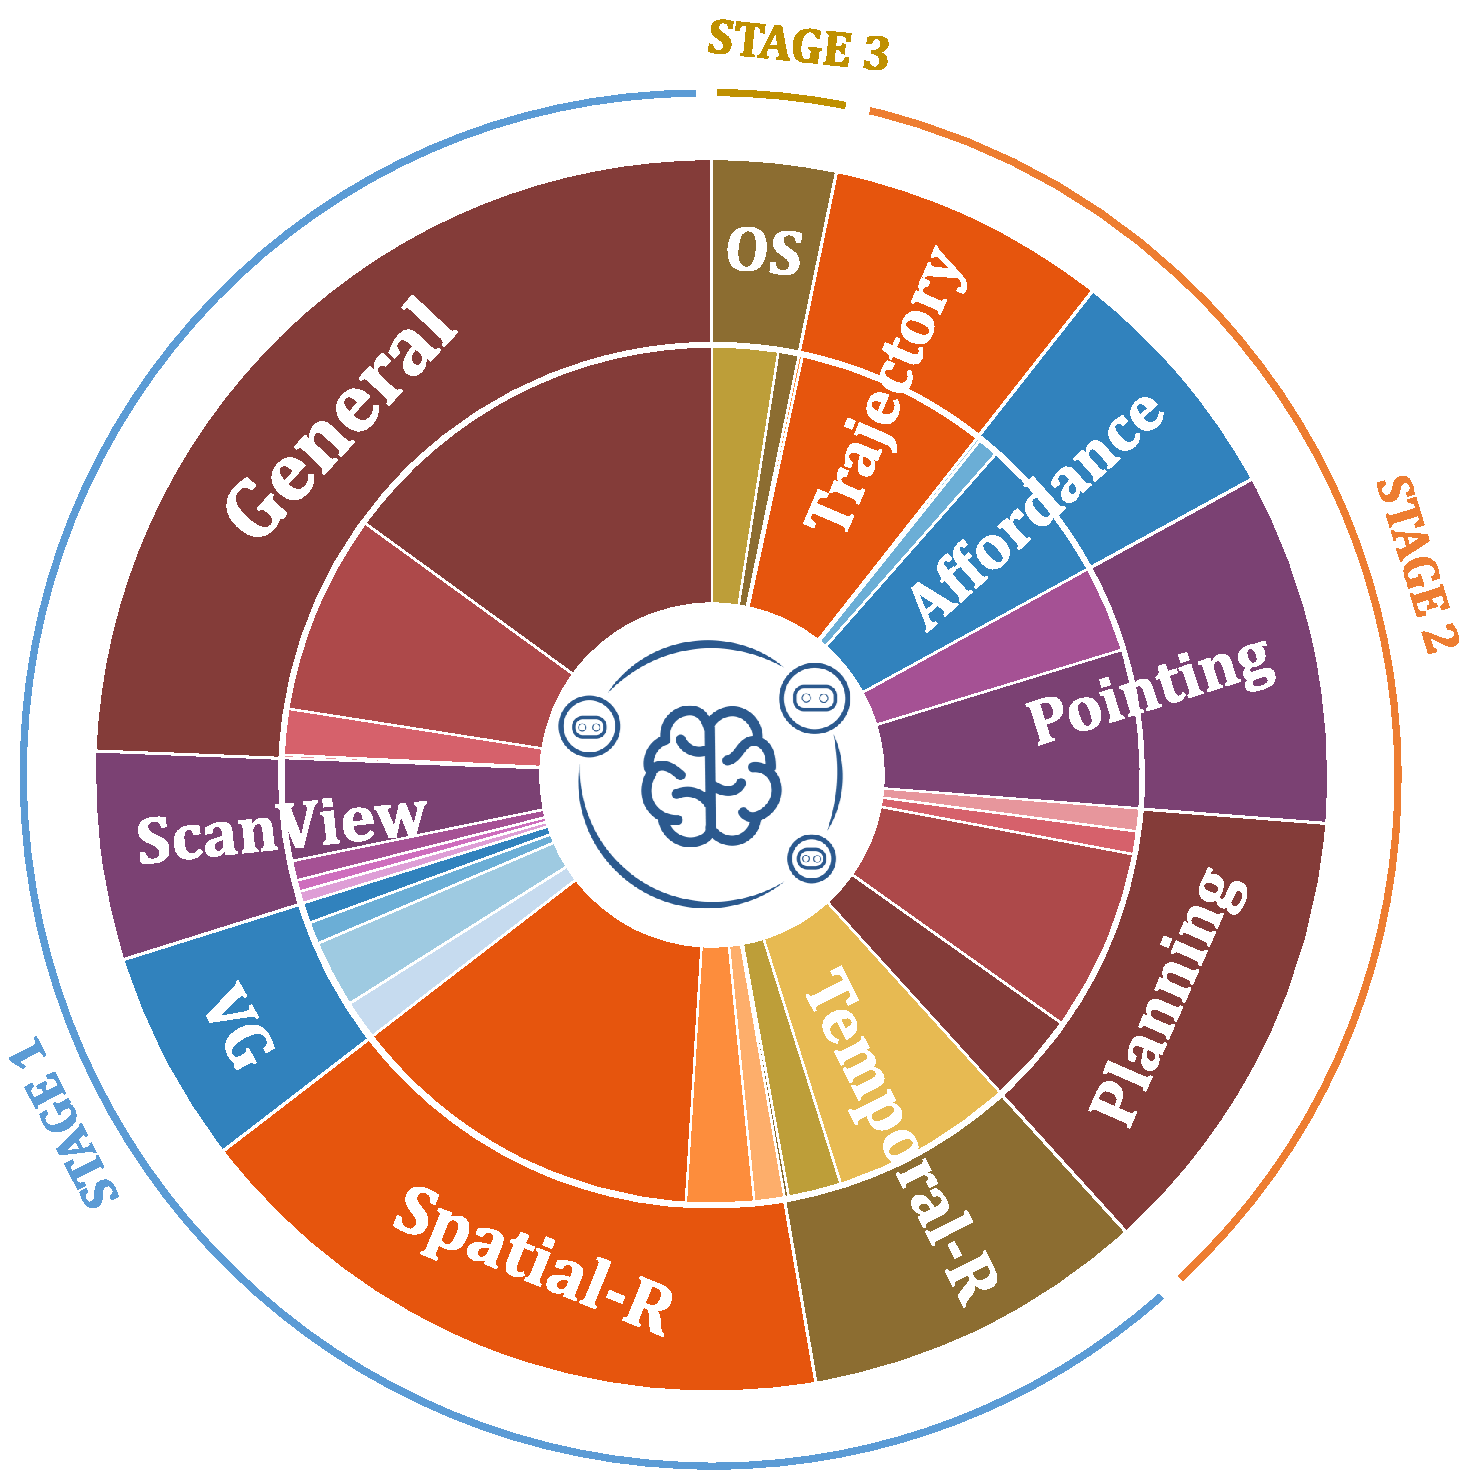
\includegraphics[width=\linewidth]{images/data.pdf}
    \caption{
        \footnotesize{\textbf{Training dataset distribution.}}
    }
    \vspace{-0.3cm}
    \label{fig:data}
\end{wrapfigure}
\textbf{Dataset Details} 
As shown in Fig.~\ref{fig:data}, the dataset for training the RoboBrain-1.5-OS model from pretrained Qwen2.5-VL-7B \cite{Qwen2.5-VL} consists of three categories: VLM datasets, Robotic datasets, and RoboOS-Enhanced datasets.
\textit{\textbf{(1) VLM Datasets:}} These are organized by capability type: General-873k \cite{li2024llavaov,liu2023mitigating} for enhancing general QA capabilities; ScanView-318k \cite{mmscan,leo,3rscan,scanqa,sqa3d} for improving multi-perspective scene perception; VG-326k \cite{li2024llavaov,yu2016modeling,mao2016generation,chen2024revisiting,krishna2017visual} for boosting visual grounding in object localization; Spatial-R-1005k \cite{yang2020graph,chen2020cops,tan2025reason} for spatial reasoning; and Temporal-R-525k \cite{zhang2025embodied,wan2022handmethat} for temporal reasoning. All data underwent rigorous cleaning to ensure the model retains strong QA abilities while enhancing localization and spatiotemporal reasoning.
\textit{\textbf{(2) Robotic Datasets:}} These were curated to target four core robotic operation capabilities: Planning, Pointing, Affordance, and Trajectory. Specifically, Planning-700k \cite{sermanet2024robovqa,ji2025robobrain,bu2025agibot} enhances long-horizon task planning; Pointing-537k \cite{deitke2024molmo,yuan2024robopoint} improves spatial position perception; Affordance-373k \cite{yuan2024robopoint,ramanathan2023paco,ji2025robobrain} predicts interactive object affordance regions; and Trajectory-428k \cite{niu2024llarva,ji2025robobrain} anticipates complete manipulation trajectories for successful execution.
\textit{\textbf{(3) RoboOS-Enhanced (OS) Datasets:}} We \textit{Multi-Robot Task Planning} and \textit{Agent-Based Tool Invocation} within the RoboOS framework. Specifically, we designed 68 multi-robot collaboration task types across supermarket, household, and restaurant scenarios, generating 45,000 samples using DeepSeek-V3 \cite{liu2024deepseek}. This dataset, named Multi-Robot-45k, features instances where each question includes a detailed scene graph, robot specifications, and a long-horizon collaborative task, while the corresponding answers provide reasoning processes and workflow graphs of decomposed subtasks. Additionally, we constructed Robotic-Agent-144k by generating correct Observation-Action pairs (positive samples) alongside probabilistically sampled error-injected Observation-Action pairs (negative samples) for each subtask from Multi-Robot-45k.

\textbf{Training Strategy}  
The training of the RoboBrain-1.5-OS model consists of three stages, as illustrated in Fig.~\ref{fig:data}. In STAGE-1, we utilize large-scale, high-quality VLM datasets with 3M samples to enhance foundational perception and reasoning. STAGE-2 employs carefully sampled robotic datasets to improve the model's four core embodied capabilities, incorporating 10\% of STAGE-1 data to prevent catastrophic forgetting, resulting in 2.3M samples. Finally, in STAGE-3, we apply RoboOS-Enhanced datasets for adaptability, mixing 2\% of STAGE-1 and 3\% of STAGE-2 data, yielding 249k samples. Throughout training, we used the Zero3 \cite{zero} distributed strategy on 20 servers, each equipped with 8$\times$A800 GPUs, with further details available in the appendix.

\textbf{Evaluation Metrics} For multi-robot planning, we use Accuracy-Rate (AR)~\cite{zhang2024lmms} to evaluate agent-based tool-calling in RoboOS. For pointing prediction, we employ the Where2Place benchmark~\cite{yuan2024robopoint} with AR to measure hit accuracy against target masks. For affordance and trajectory prediction, we evaluate using ShareRobot~\cite{ji2025robobrain} benchmark, where affordance is measured by mAP across IoU thresholds, while trajectory prediction uses Discrete Fréchet Distance (DFD)~\cite{gu2023rt}, Hausdorff Distance (HD), and RMSE for macroscopic and microscopic analysis. To better evaluate autonomous trajectory prediction, we removed the initial start-point hints during trajectory assessment.

\subsection{Results on Embodied Evaluation}
To evaluate the embodied capabilities of RoboBrain-1.5-OS—the core component of RoboOS—we selected comparable VLMs (\textit{e.g.}, LLaVA-OneVision-7B~\cite{li2024llavaov}, Qwen2.5-VL-7B~\cite{Qwen2.5-VL}) with similar parameter scales, alongside larger LLMs (\textit{e.g.}, Qwen3-14B~\cite{qwen3_2025}, DeepSeek-V3-685B~\cite{liu2024deepseek}) as general baselines. We also compared against embodied baselines such as RoboPoint-14B~\cite{yuan2024robopoint} and RoboBrain-1.0~\cite{ji2025robobrain}. As shown in Tab.~\ref{tab:main_tab}, RoboBrain-1.5-OS achieves outstanding performance in multi-robot planning, surpassing Qwen2.5-VL-7B by 28.14\% and outpacing DeepSeek-V3-685B by 5.53\%, thereby enhancing RoboOS's capabilities. It also outperforms all baselines in pointing, affordance, and trajectory prediction, improving over RoboBrain-1.0 by 3.64\%, 16.96\%, and 40.77\%, respectively, demonstrating superior results across multiple embodied capabilities.

\begin{table*}[t]
    \centering
    \caption{\textbf{Performance across four key embodied capabilities.} Top results are highlighted in \textbf{bold}.}
    \vspace{0.2cm}
    \resizebox{\textwidth}{!}{
    \begin{tabular}{l|cccc|ccc|c|ccc}
        \toprule
        \multicolumn{1}{l|}{\multirow{2}{*}{\textbf{Models / Metrics}}} & \multicolumn{4}{c|}{\textbf{Multi-Robot Planning}} & \multicolumn{3}{c|}{\textbf{Pointing}} &  \multicolumn{1}{c|}{\textbf{Affordance}} &  \multicolumn{3}{c}{\textbf{Trajectory}}\\ 
        \cmidrule(lr){2-5} \cmidrule(lr){6-8} \cmidrule(lr){9-9} \cmidrule(lr){10-12}
        & \textbf{Rest.} & \textbf{House.} &\textbf{Super.} &\textbf{AVG $\uparrow$} & \textbf{Seen} & \textbf{Unseen} & \textbf{AVG $\uparrow$} & \textbf{mAP $\uparrow$} & \textbf{DFD $\downarrow$} & \textbf{HD $\downarrow$} & \textbf{RMSE $\downarrow$} \\ 
        \midrule
        \rowcolor[HTML]{F2F2F2} \multicolumn{12}{l}{\textbf{General Baselines}} \\ \midrule
        Llava-OneVision-7B~\cite{li2024llavaov}             & 11.31 & 8.26 & 9.33 & 9.63 & 55.54 & 48.48 & 53.42 & 11.37 & 0.3558 & 0.3310 & 0.2749 \\
        Qwen2.5-VL-7B~\cite{Qwen2.5-VL}           & 43.22 & 59.30 & 58.29 & 53.60 & 57.20 & 47.60 & 54.32 & 14.06 & 0.2964 & 0.2751 & 0.2254 \\
        Qwen3-14B~\cite{qwen3_2025} & 47.74  & 63.82  & 43.22  & 51.60  & $\times$ & $\times$ & $\times$ & $\times$ & $\times$ & $\times$  & $\times$ \\
        DeepSeek-V3-685B~\cite{liu2024deepseek} & 69.85 & 83.92 & 74.87 & 76.21  & $\times$ & $\times$ & $\times$ & $\times$ & $\times$ & $\times$  & $\times$ \\ \midrule
        \rowcolor[HTML]{F2F2F2} \multicolumn{12}{l}{\textbf{Embodied Baselines}} \\ \midrule
        RoboPoint-14B~\cite{yuan2024robopoint} & -- & -- & -- & -- & 46.77 & 44.48 & 46.08 & -- & --  & -- & -- \\ 
        RoboBrain-7B-1.0~\cite{ji2025robobrain} & 17.59 & 12.06 & 10.55 & 13.40 & 54.64 & 49.45 & 53.09  & 27.10 & 0.1910 & 0.1710 & 0.1330 \\ 
        \rowcolor[HTML]{DAEFF9} RoboBrain-7B-1.5-OS & \textbf{78.39} & \textbf{86.93} & \textbf{79.90} & \textbf{81.74} & \textbf{57.23} & \textbf{55.57} & \textbf{56.73} & \textbf{44.06} & \textbf{0.0994} & \textbf{0.0966} & \textbf{0.0801} \\
        \bottomrule
    \end{tabular}
    }
    \label{tab:main_tab}
\vspace{-0.5em}
\end{table*}

\subsection{Demos on Real-World Collaboration}  
To demonstrate RoboOS's multi-robot collaboration, we present demos in restaurant, household, and supermarket settings. In the restaurant scenario (Fig.~\ref{fig:demo}~(a)), a Unitree G1 humanoid robot and an Agilex dual-arm robot work together to fulfill the task: ``I'm hungry and order a normal burger.'' RoboBrain-1.5-OS handles scene-aware reasoning, decomposing the task into subtasks for burger preparation and delivery.
In the household scenario (Fig.~\ref{fig:demo}~(b)), a Realman single-arm robot and an Agilex dual-arm robot collaborate to accomplish tasks like ``Give me an orange and a knife.'' 
In the supermarket (Fig.~\ref{fig:demo}~(c)), RoboBrain-1.5-OS assists a customer with gift selection by analyzing dimensions and bag compatibility. It coordinates the Realman and Agilex robots, with the Agilex executing a VLA-cerebellum skill to ``open the gift bag,'' while the Realman selects and places the gift.
Future applications may explore more complex collaborations with three or more robots, significantly advancing embodied AI and robotics.

\begin{figure*}[t]
    \centering
    \vspace{-0.2cm}
    
\includegraphics[width=0.98\linewidth]{images/demo.pdf}
    \vspace{-0.1cm}
    \caption{
\textbf{Real-world RoboOS Demonstrations.} We showcase multi-robot collaboration in three scenarios: (a) Restaurant: Unitree G1 and Agilex robots prepare burgers. (b) Household: Realman and Agilex robots fetch items. (c) Supermarket: Robots coordinate gift selection and packaging.
    }
       \vspace{-0.5cm}
    \label{fig:demo}
\end{figure*}
